\chapter{Конструкторская часть}

В этой части представляются требования к программе, алгоритм визуализации сцены, выбранные типы и структуры данных, диаграмма классов.

\section{Требования к программе}

Программа должна обладать графическим интерфейсом, который позволит пользователю:
\begin{itemize}[label=--]
	\item изменять геометрические и спектральные характеристики модели многогранника;
	\item изменять положение модели многогранника в пространстве;
	\item изменять положение камеры в пространстве;
	\item изменять режим отображения сцены между <<каркасным>>, отображающим каркасы моделей, <<реалистичным>>, отображающим линии пересечения моделей, <<световым>>, отображающим сцену с учётом освещения и <<теневым>>, отображающим сцену с тенями, возникающими от освещения.
\end{itemize}

Разработанная программа должна выполнять следующие требования:
\begin{itemize}[label=--]
	\item источник света должен создаваться при запуске;
	\item в пространстве может быть только один источник света;
	\item в пространстве может быть только одна камера;
	\item программа обязана правильно обрабатывать некорректные вводимые данные.
\end{itemize}

\section{Общий алгоритм визуализации сцены}

На рисунке~\ref{fig:scene-visualization} представлен алгоритм, который генерирует изображение. Он принимает на вход геометрические и спектральные параметры моделей, характеристики камеры, данные об источнике света и его спектральные свойства, а на выходе предоставляет визуализированную сцену на экране.

\begin{figure}[h] 
	\centering
	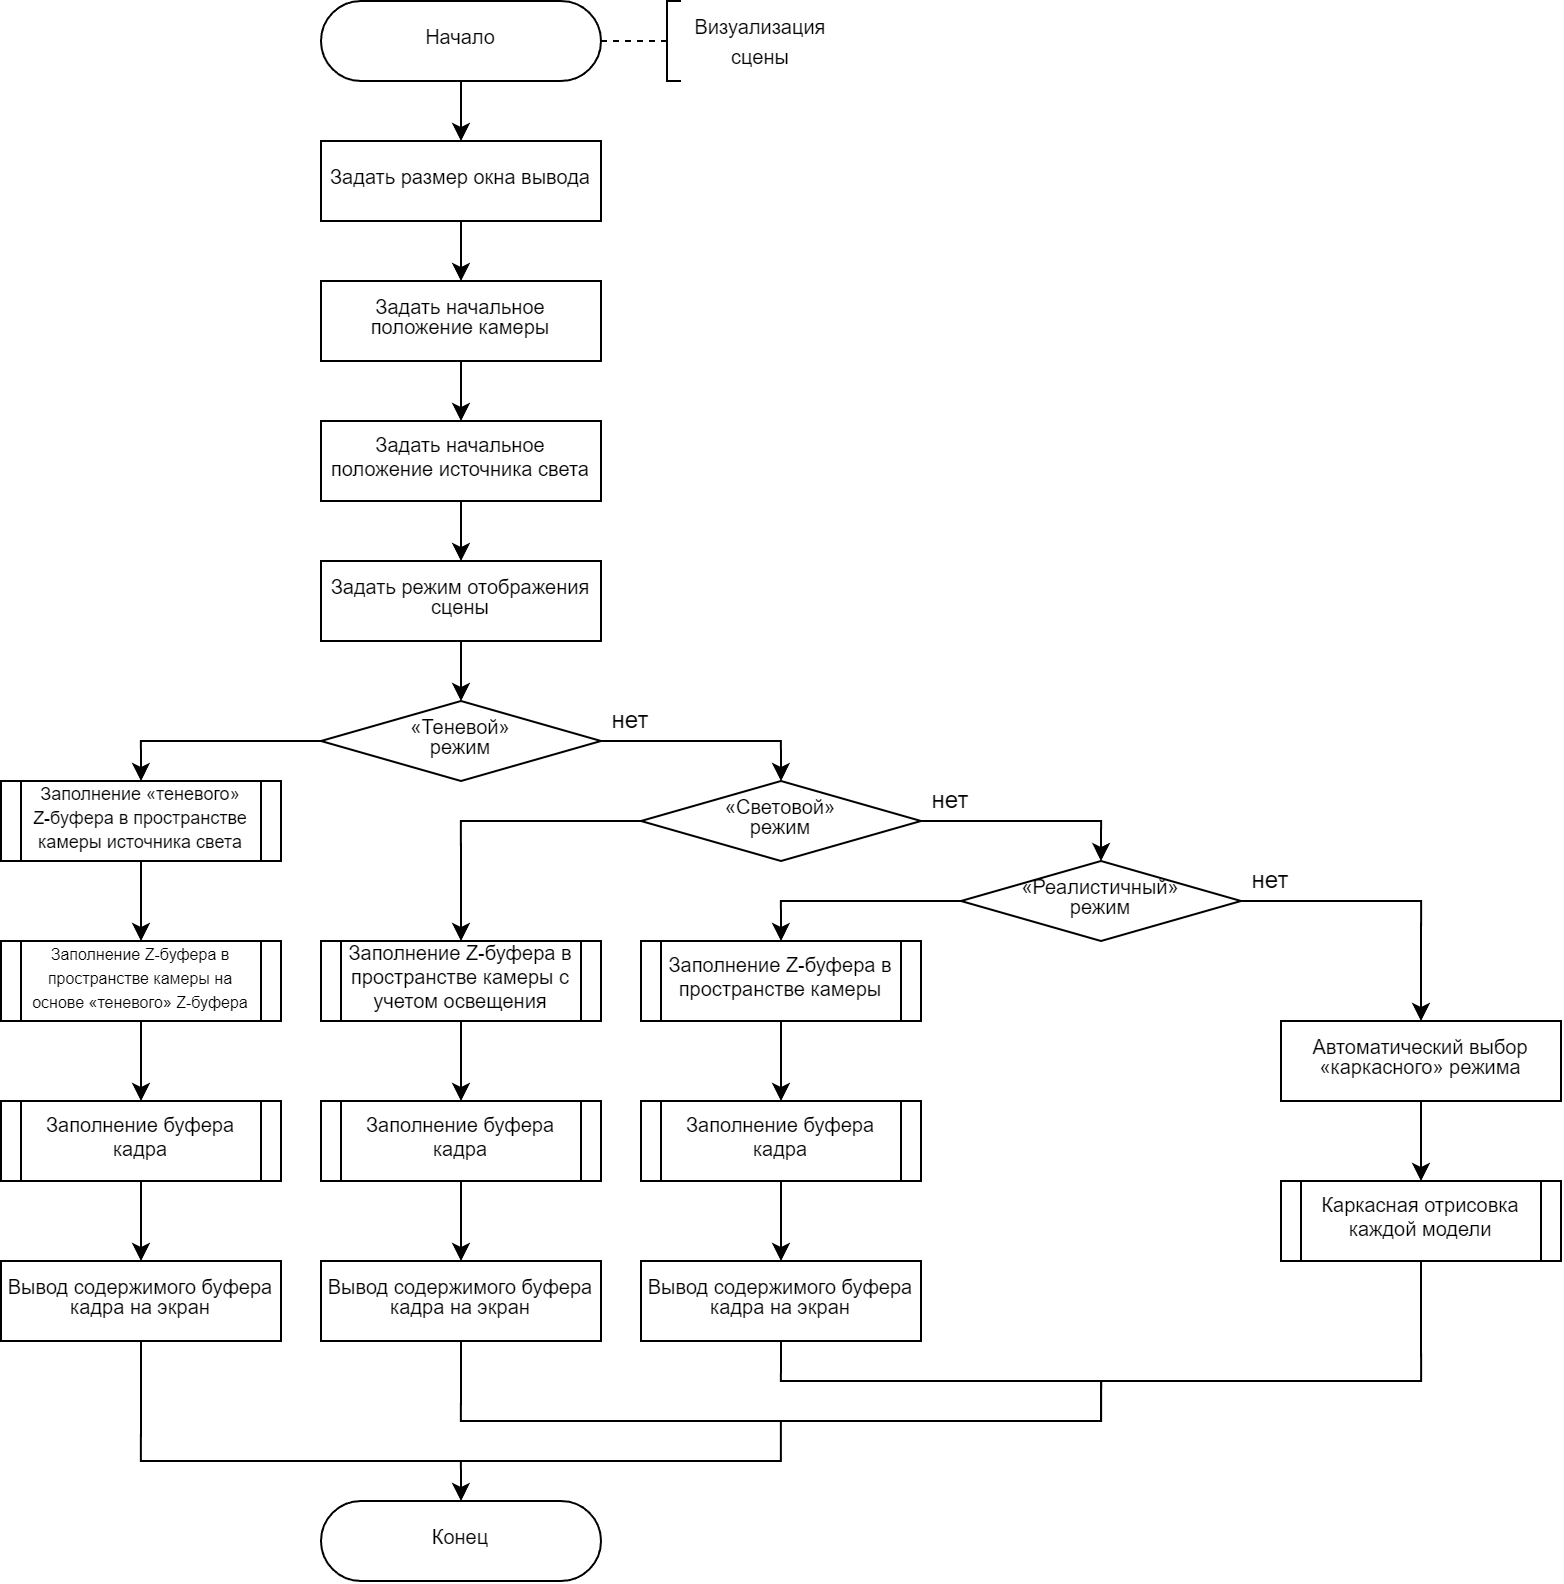
\includegraphics[width=1\textwidth]{images/scene-visualization.png}
	\caption{Общий алгоритм визуализации сцены} 
	\label{fig:scene-visualization} 
\end{figure}

\clearpage

Более подробный алгоритм визуализации сцены в <<теневом>> режиме отображения сцены при инициализированной сцене представлен на рисунке~
\ref{fig:shadow-mod}.
\begin{figure}[h] 
	\centering
	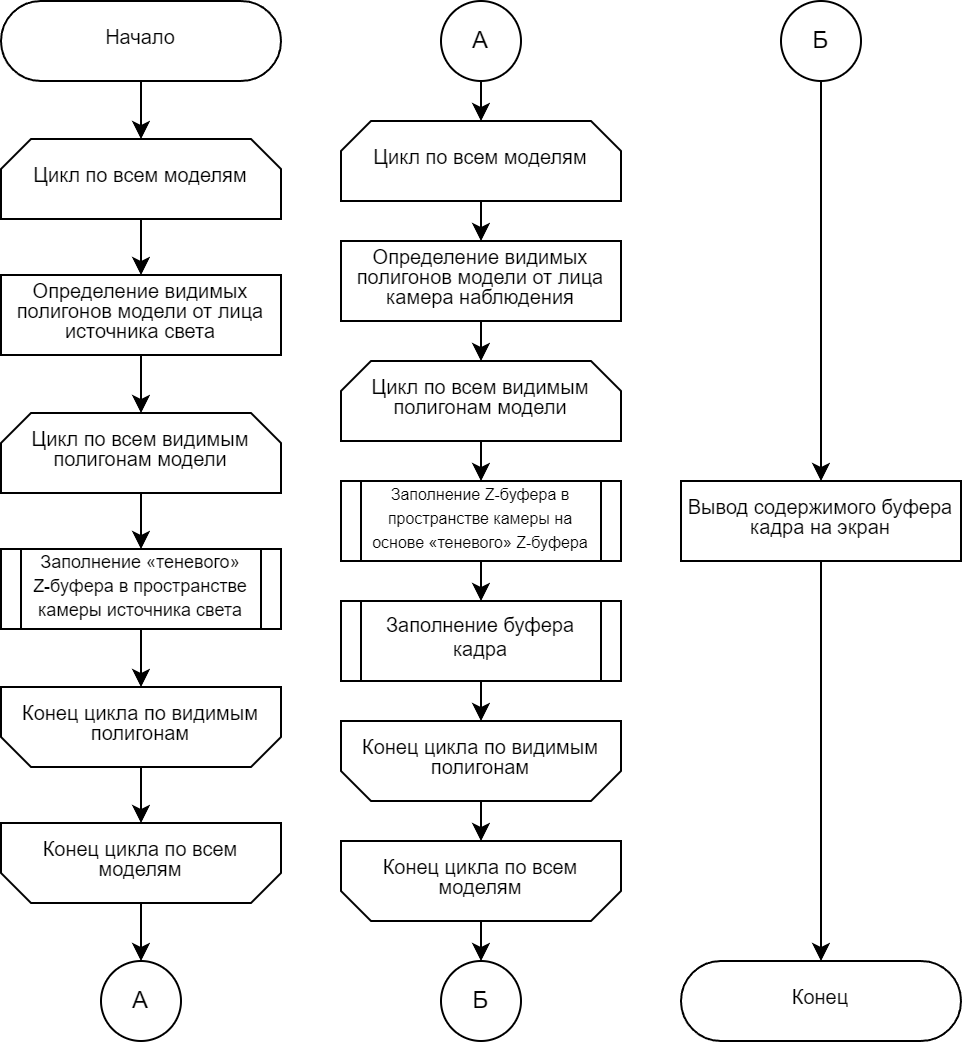
\includegraphics[width=1\textwidth]{images/shadow-mod.png}
	\caption{Общий алгоритм визуализации сцены в <<теневом>> режиме при инициализированной сцене} 
	\label{fig:shadow-mod} 
\end{figure}

\clearpage

Более подробный алгоритм визуализации сцены в <<световом>>, <<реалистичном>> и <<каркасном>> режимах отображения сцены при инициализированной сцене представлены на рисунке~\ref{fig:other-mods}.
\begin{figure}[h] 
	\centering
	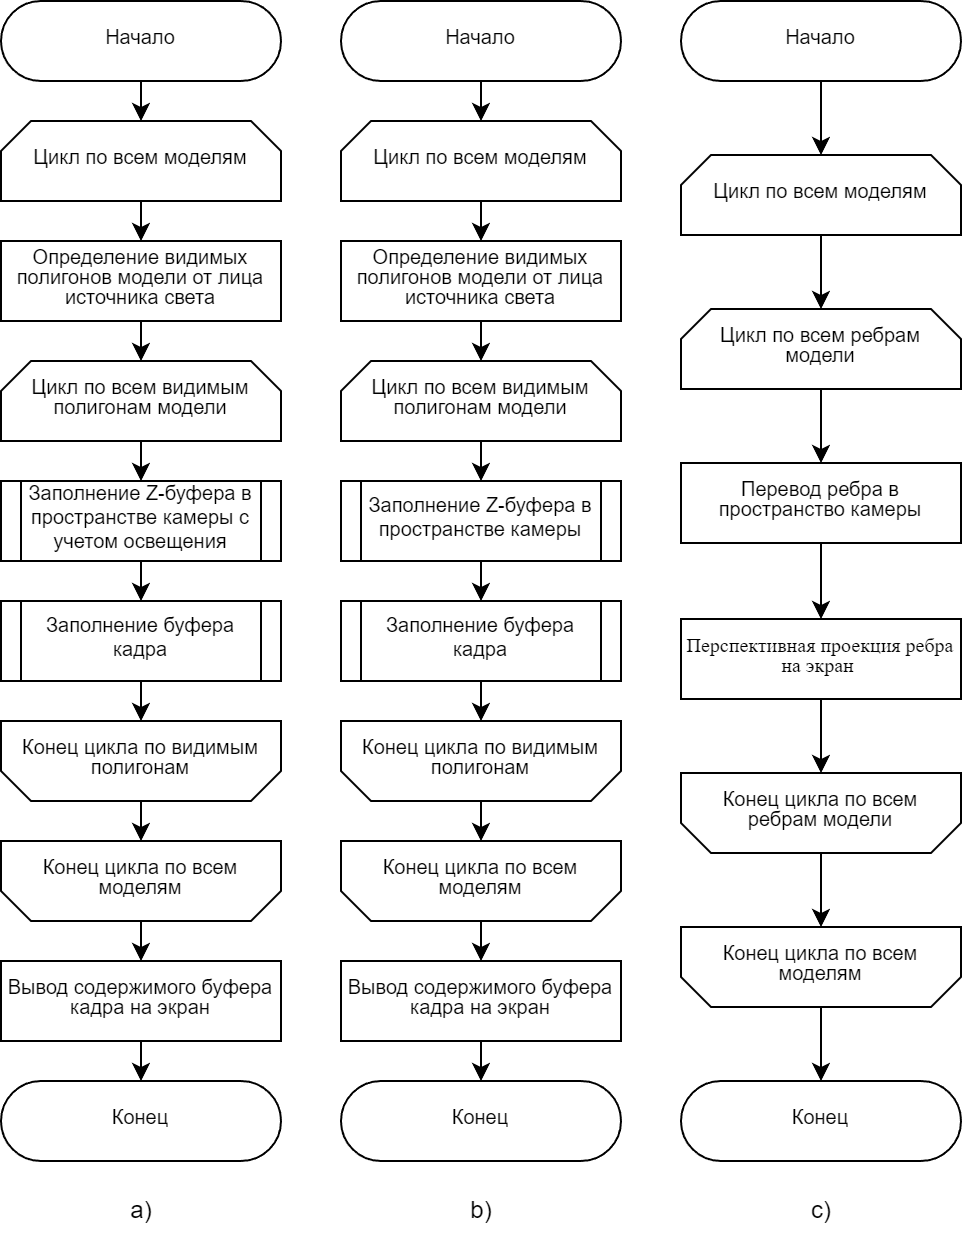
\includegraphics[width=0.8\textwidth]{images/other-mods.png}
	\caption{Общий алгоритм визуализации сцены в иных режимах при инициализированной сцене: <<световой>> (a), <<реалистичный>> (b), <<каркасный>> (c)} 
	\label{fig:other-mods} 
\end{figure}

\clearpage

\section{Афинные преобразования}

Для изменения положения модели в пространстве можно использовать следующие преобразования: перемещение и поворот. Каждое из этих преобразований может быть представлено в виде матрицы:
\begin{enumerate}
	\item перемещение вдоль координатных осей $O_X$, $O_Y$ и $O_Z$ соответственно на величины $d_x$, $d_y$, $d_z$:
	\begin{equation}
		\begin{pmatrix}
			1 & 0 & 0 & 0 \\
			0 & 1 & 0 & 0 \\
			0 & 0 & 1 & 0 \\
			d_x & d_y & d_z & 1
		\end{pmatrix}
	\end{equation}
	\item поворот вокруг координатных осей $O_X$, $O_Y$ и $O_Z$ на угол $\theta$:
	\begin{equation}
		R = R_X \cdot R_Y \cdot R_Z
	\end{equation}
	где $R$ -- матрица поворота, $R_X$ матрица поворота вокруг оси $O_X$ на угол $\theta$, $R_Y$ -- матрица поворота вокруг оси $O_Y$ на угол $\theta$, $R_Z$ -- матрица поворота вокруг оси $O_Z$ на угол $\theta$.
	\begin{itemize}[label=--]
		\item поворот вокруг оси $O_X$ на угол $\theta$:
		\begin{equation}
			\begin{pmatrix}
				1 & 0 & 0 & 0 \\
				0 & cos(\theta) & sin(\theta) & 0 \\
				0 & -sin(\theta) & cos(\theta) & 0 \\
				0 & 0 & 0 & 1
			\end{pmatrix}
		\end{equation}
		\item поворот вокруг оси $O_Y$ на угол $\theta$:
		\begin{equation}
			\begin{pmatrix}
				cos(\theta) & 0 & -sin(\theta) & 0 \\
				0 & 1 & 0 & 0 \\
				sin(\theta) & 0 & cos(\theta) & 0 \\
				0 & 0 & 0 & 1
			\end{pmatrix}
		\end{equation}
		\item поворот вокруг оси $O_Z$ на угол $\theta$:
		\begin{equation}
			\begin{pmatrix}
				cos(\theta) & sin(\theta) & 0 & 0 \\
				-sin(\theta) & cos(\theta) & 0 & 0 \\
				0 & 0 & 1 & 0 \\
				0 & 0 & 0 & 1
			\end{pmatrix}
		\end{equation}
	\end{itemize}
\end{enumerate}

\section{Камера}

Камера отвечает за захват и отображение части трёхмерной сцены на двумерную поверхность. Она определяет, как объекты будут видны зрителю, а также управляет параметрами визуализации, такими как угол обзора.

\subsection{Пирамида видимого пространства}

Пирамида видимого пространства (\textit{англ. viewing frustum}) представляет собой объем, в пределах которого объекты могут быть видимы камерой. Этот объем имеет форму усеченной пирамиды (рис. \ref{fig:viewing-frustum}) и определяется несколькими ключевыми параметрами:
\begin{itemize}[label=--]
	\item ближняя плоскость: плоскость, находящаяся на определенном расстоянии от камеры, перед которой объекты начинают отображаться. Объекты, находящиеся ближе, не будут видны;
	\item дальняя плоскость: плоскость, за которой объекты не отображаются;
	\item поле зрения (\textit{англ. field of view}): угол, под которым камера охватывает сцену. Поле зрения влияет на то, насколько широко камера может видеть, и определяет степень искажения объектов в зависимости от их расстояния до камеры.
\end{itemize}

Пирамида видимого пространства позволяет игнорировать объекты вне этого объема, что увеличивает скорость рендеринга.

\clearpage

\begin{figure}[h] 
	\centering
	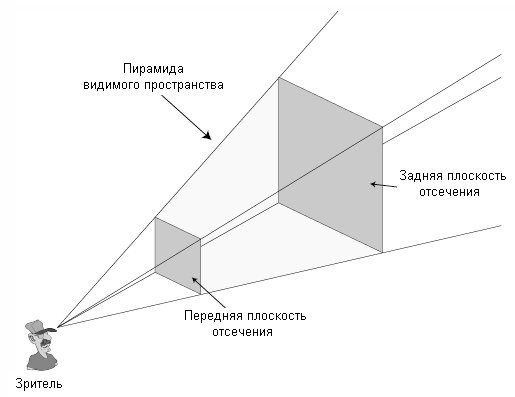
\includegraphics[width=0.7\textwidth]{images/viewing-frustum.png}
	\caption{Пирамида видимого пространства} 
	\label{fig:viewing-frustum} 
\end{figure}

\subsection{Пространство модели}

Пространство модели -- это локальная система координат, в которой располагается конкретный объект сцены. В этом пространстве объект имеет координаты, которые определяют его положение, ориентацию и масштаб относительно своей собственной системы координат. 

Пусть вершина $V_L$ имеет однородные координаты $x_L, y,_L z_L, 1$ в пространстве модели, тогда её можно описать с помощью матрицы:
\begin{equation}
	V_L = 
	\begin{pmatrix}
		x_L \\
		y_L \\
		z_L \\
		1
	\end{pmatrix}
	\label{eq:local-vertex}
\end{equation}

\subsection{Мировое пространство}

Мировое пространство — это система координат, в которой расположены все объекты сцены. В этом пространстве каждое тело имеет свои координаты, определяющие его положение, ориентацию и масштаб. Мировое пространство позволяет организовать объекты в сцене.

Для перевода модели из её пространства в мировое нужно получить матрицу перевода $W$. Для её формирования необходимо составить матрицу перемещения модели относительно начала мировой системы координат $M_W$ и матрицу поворота модели относительно её центра $R_W$.
\begin{equation}
	W = M_W \cdot R_W
\end{equation}
где $W$ -- матрица перевода модели из её пространства в мировое, $M_W$ -- матрица перемещения, $R_W$ -- матрица поворота.

Чтобы перевести вершину $V_L$ (\ref{eq:local-vertex}) из её локального пространства в мировое, её нужно умножить на матрицу перевода $W$:
\begin{equation}
	V_W = W \cdot V_L
	\label{eq:world-vertex}
\end{equation}
где $V_W$ -- матричная запись вершины $V_L$, переведённой из её локального пространства в мировое и имеющей однородные координаты $x_W, y_W, z_W, w_W$, $W$ -- матрица перевода модели из её пространства в мировое.

\subsection{Пространство камеры}

Пространство камеры — это система координат, в которой камера воспринимает объекты. Оно определяется положением и ориентацией камеры в мировом пространстве. Основные компоненты пространства камеры включают:

\begin{itemize}[label=--]
	\item положение камеры $P$: определяет, где находится камера в мировом пространстве;
	\item ориентация камеры $\vec{D}$: направление взгляда камеры, задаваемое вектором;
	\item cистема координат $\vec{D}, \vec{U}, \vec{R}$: устанавливает оси $O_X$, $O_Y$ и $O_Z$ для камеры, где ось $\vec{D}$ направлена вперед (ампликата), ось $\vec{U}$ -- вверх (ордината), а ось $\vec{R}$ -- вправо (абсцисса).
	\begin{equation}
		\vec{R} = \vec{D} \times O_Y \\
	\end{equation}
	\begin{equation}
		\vec{U} = \vec{D} \times \vec{R}
	\end{equation}
\end{itemize}

Для перевода модели из мирового пространства в пространство камеры нужно получить матрицу перевода $C$. Для её формирования необходимо составить матрицу перемещения камеры относительно начала мировой системы координат $M_C$ и матрицу поворота камеры в мировом пространстве $R_C$.
\begin{equation}
	M_C = 
	\begin{pmatrix}
		1 & 0 & 0 & 0 \\
		0 & 1 & 0 & 0 \\
		0 & 0 & 1 & 0 \\
		-P_x & -P_y & -P_z & 1
	\end{pmatrix}
\end{equation}
где $M_C$ -- матрица перемещения камеры относительно начала мировой системы координат, $P$ -- положение камеры в мировом пространстве.

\begin{equation}
	R_C = 
	\begin{pmatrix}
		\vec{R}_x & \vec{U}_x & \vec{D}_x & 0 \\
		\vec{R}_y & \vec{U}_y & \vec{D}_y & 0 \\
		\vec{R}_z & \vec{U}_z & \vec{D}_z & 0 \\
		0 & 0 & 0 & 1 
	\end{pmatrix}
\end{equation}
где $R_C$ -- матрица поворота камеры в мировом пространстве, $\vec{R}$ -- абсцисса системы координат камеры, $\vec{U}$ -- ордината системы координат камеры, $\vec{D}$ -- направление взгляда камеры (ампликата системы координат камеры).

\begin{equation}
	C = M_C \cdot R_C
\end{equation}
где $C$ -- матрица перевода модели из мирового пространства в пространство камеры, $M_C$ -- матрица перемещения камеры относительно начала мировой системы координат, $R_C$ -- матрица поворота камеры в мировом пространстве.

Чтобы перевести вершину $V_W$ (\ref{eq:world-vertex}) из мирового пространства в пространство камеры, её нужно умножить на матрицу перевода $C$:
\begin{equation}
	V_C = C \cdot V_W
\end{equation}
где $V_C$ -- матричная запись вершины $V_W$, переведённой из мирового пространства в пространство камеры и имеющей однородные координаты $x_C, y_C, z_C, w_C$, $C$ -- матрица перевода модели из мирового пространства в пространство камеры. 

\subsection{Перспективная проекция}

...

\section{Невидимые грани}

...

\section{Схемы алгоритмов}

...

\section{Выбор типов и структур данных}

...

\section{Диаграмма классов}

...

\section{Вывод}

<что сделали в конструкторке и получили в результате, кратко>

\clearpage
